

% Document for tutorial 4
\documentclass[12pt]{article}
\usepackage{graphicx}
\title{Tables and figures}

\author{John Doe}
\begin{document}
\maketitle

Example of picture inclusion:
\begin{center}
	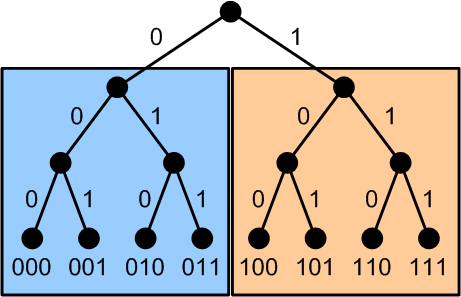
\includegraphics[width=0.5\textwidth]{tree}
\end{center}


Example of picture inclusion:
\begin{center}
	\fbox{
		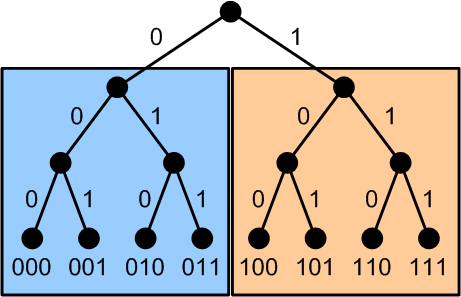
\includegraphics[width=0.5\textwidth]{tree}
	}
\end{center}


\begin{table}[ht]
	\caption{My little table}
	\begin{center}
		\begin{tabular}{clr} \hline
			centred & left & right \\ \hline\hline
			C & L & R \\
			111 & 222 & 333 \\ \hline
		\end{tabular}
	\end{center}
\end{table}


\begin{figure}[ht]
	\begin{center}
		\fbox{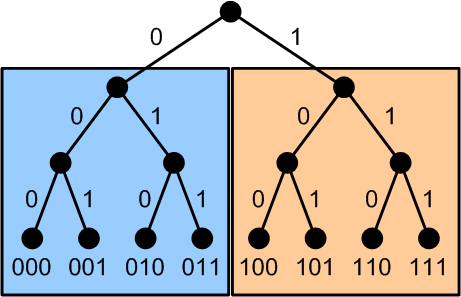
\includegraphics[width=0.5\textwidth]{tree}}
	\end{center}
	\caption{My little figure}
\end{figure}


\begin{figure}[ht]
	\centering
	\fbox{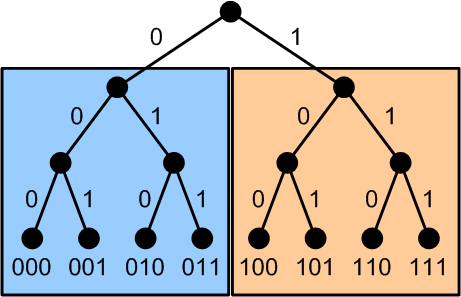
\includegraphics[width=0.5\textwidth]{tree}}
	\caption{My little figure}
\end{figure}



\label{blabla} to create a label named blabla,
\ref{blabla} to reference the label named blabla



\section{A section} \label{melabel}
We will say more in section~\ref{othersec}
about figure~\ref{myfig}\ldots{}
\begin{figure}[ht]
	\centering
	\fbox{
		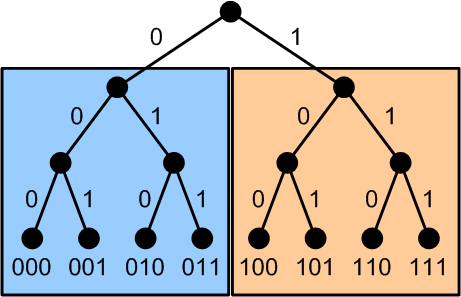
\includegraphics[width=0.5\textwidth]{tree}
	}
	\caption{My little figure} \label{myfig}
\end{figure}
\section{Another section} \label{othersec}
As mentioned in section~\ref{melabel}
on page~\pageref{melabel}\ldots{}

\end{document}
